\section{선행연구에서 수집한 자료의 재범주화 및 비교분석}

내용 작성

\section{챗봇 개발}

\subsection{LLM에 RAG를 적용한 생성형 AI 챗봇 개발 사례}

내용 작성

\subsection{프로토타입 개발 과정}

그림 삽입 예시

PDF를 그림으로 넣어도 되고, png 파일을 넣어도 됩니다. 파워포인트로 그린 그림을 PDF로 저장한 그림을 넣는 예시입니다.

표와 그림은 모두 Cref로 언급하면 자동으로 표와 그림을 나누어 번호가 매겨집니다.

챗봇 프로토타입 개발 과정에서 LLM에 RAG를 적용하여 답변을 생성하는 과정을 개략적으로 나타내면 \Cref{method-RAG}\와 같다.

\begin{figure}[h!]
    \centering
    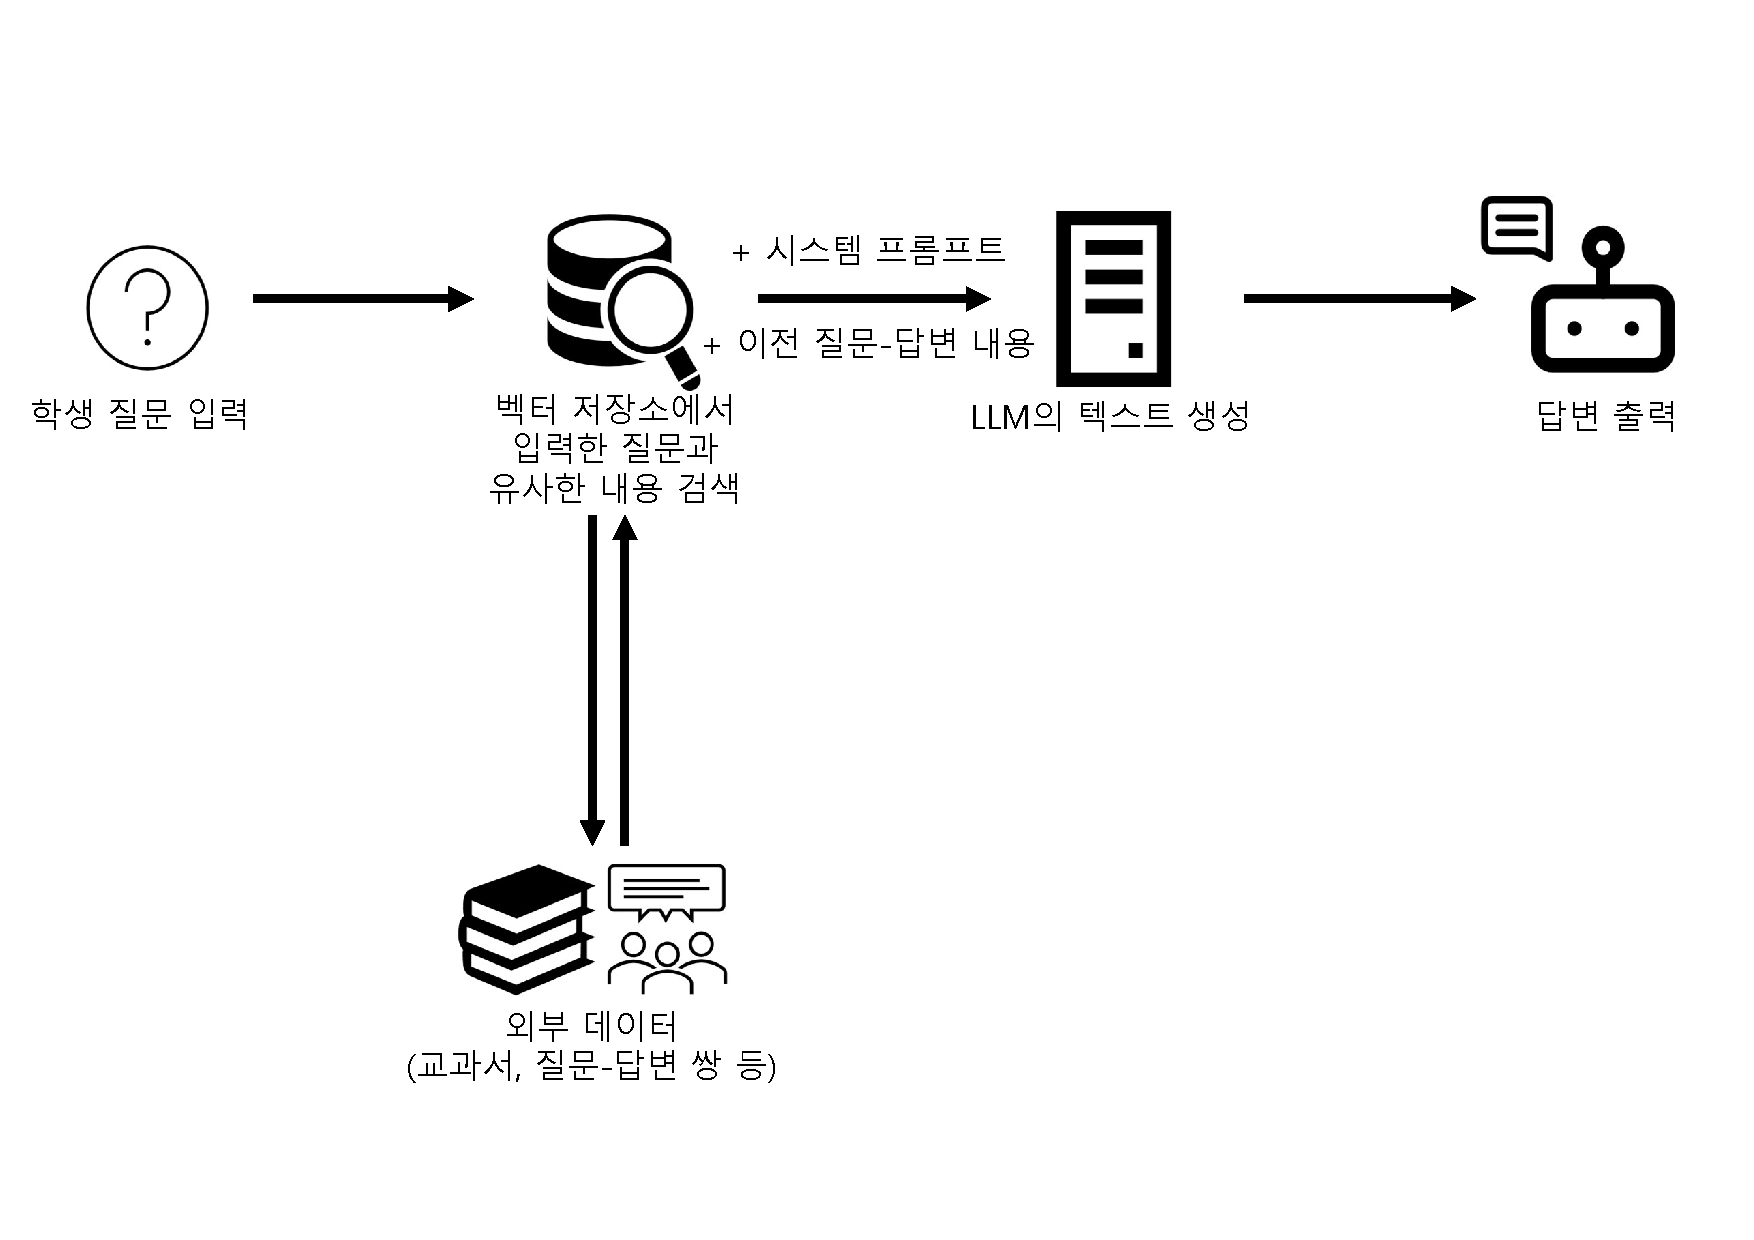
\includegraphics[width=12cm]{pdfs/method-RAG.pdf}
    \caption{LLM에 RAG를 적용하여 답변을 생성하는 과정}
    \label{method-RAG}
\end{figure}

/figs 폴더에도 그림을 넣어서 사용했습니다. 이 디렉토리는 비워두겠습니다.

\subsubsection{subsubsection도 넣을 수 있어요}

...

\subsubsection{subsubsection도 넣을 수 있어요}

...

\subsubsection{subsubsection도 넣을 수 있어요}

\cite{min2024}\가 ... 처럼 쓰면 이/가도 자동으로 바뀝니다.

\subsubsection{subsubsection도 넣을 수 있어요}

강조용 글꼴 변화는 texttt를 사용하세요.

PDF 파일을 불러온 내용을 내용을 일반적인 문장으로 만들기 위해 \texttt{$\backslash$x}로 시작하는 ... 부분을 제외하고자 \texttt{진도체크, 보고서 작성하기, 도움 영상, 발표하기, 고르시오, ㄱ, ㄴ, ㄷ, 만들어 보자, 평가하기} 등 총 50가지 정도의 문구가 있는 문장을 삭제했다.

...

\subsubsection{시스템 프롬프트 구성}

컴퓨터 코드 삽입 예시

2024년 9월에 최종적으로 수정한 시스템 프롬프트는 \Cref{gen-prompt-new}\와 같다.

\begin{figure}[h!]
    \begin{lstlisting}
        template = '''[BOS]system
        당신은 고등학교 과학 선생님입니다. 학생들의 질문에 200 단어 이내의 한국어로만 답변해야 합니다.
        중요: 다음 규칙을 반드시 따르세요.
        1. 출력 관련 지시사항:
        (1) Markdown 을 써서 가독성을 높이세요.
        (2) 모든 수식은 무조건 이중 '$' 기호로 감싸서 출력해야만 합니다. 예: $$ 3 mol $$
        (3) http 나 https 로 시작하는 URL 은 무조건 plain text 로 표현하세요 !
        2. 학생이 입력한 질문이 " 안녕하세요 ? ", " 안녕 ? ", " 고마워 ", " 감사합니다 " 와 같은 인사나 감사 표현이라면:
        (1) HISTORY 와 CONTEXT 를 완전히 무시하세요.
        (2) 오직 해당 인사에 대해서만 간단히 응답하세요.
        (3) 이 경우, ' 생각 '과 ' 답변 ' 구조를 사용하지 마세요.
        3. 그밖의 모든 질문에 대해서는:
        (1) ' 생각 '과 ' 답변 ' 두 부분으로 나누어 응답하세요.
        (2) CONTEXT 와 HISTORY 로부터 답변할 수 있는 경우 가장 우선적으로 참조하여 답변하세요.
        (3) 관련 정보가 없는 경우, 자체 지식을 사용하세요.
        (4) 답변할 수 없는 경우 " 죄송합니다. 제가 알지 못하는 내용입니다. "라고 말하세요.
        (5) 고등학교 1 학년 학생이 이해할 수 있는 적절한 용어를 사용하세요.
        HISTORY: {history}
        CONTEXT: {context}
        HUMAN: {question}
        [|endofturn|]
        [BOS]human
        {question}
        [|endofturn|]
        [BOS]assistant
        
        [|endofturn|]'''
    \end{lstlisting}
    \caption{교사와 학생의 평가를 반영하여 개선한 시스템 프롬프트}
    \label{gen-prompt-new}
\end{figure}

표 작성 예시

표와 그림은 모두 Cref로 언급하면 자동으로 표와 그림을 나누어 번호가 매겨집니다.

두 가지 학교 맞춤형 과학 질문-답변 챗봇의 사용 기록 및 사용자 평가 내용의 개요는 \Cref{methods-comparison-verdict}\와 같다.

\begin{table}
    \centering
    \caption{두 가지 학교 맞춤형 과학 질문-답변 챗봇의 사용 기록 및 사용자 평가 내용의 개요}
    \resizebox{0.9\textwidth}{!}{%
    \begin{tabular}{ccc}
        \hline
        범주 & 선행연구 1 & 선행연구 2 \\
        \hline
        자료 수집 기간과 학생의 챗봇 활용 관련 자료 수집 방법 & O & O \\
        학생이 주로 챗봇을 활용한 시간과 사용한 기기 & O & O \\
        학생의 질문 주제 분류 & O & O \\
        학생의 챗봇 사용상 나타나는 특징 & O & O \\
        학생의 설문조사 응답 결과 & X & O \\
        \hline
    \end{tabular}
    }
    \label{methods-comparison-verdict}
\end{table}

복잡한 표 작성 예시 1

multicolumn, multirow\를 적극적으로 활용하세요. 오류가 가장 적게 납니다.

\begin{table}[h!]
    \centering
    \caption{LLM별 RAG 적용 실험 조건}
    \begin{tabular}{ll}
    \hline
    \multicolumn{1}{c}{\textbf{오픈소스 LLM}} & \multicolumn{1}{c}{\textbf{실험 조건}} \\ \hline
    LG EXAONE 3.0 7.8B &
    \begin{tabular}{l}
    1. 교사용 교과서와 질문-답변 쌍 모두 활용 \\
    2. 교사용 교과서만 활용 \\
    3. 질문-답변 쌍만 활용 \\
    4. RAG 적용 안 함
    \end{tabular} \\ \hline
    Google Gemma 2 9B & 
    \begin{tabular}{l}
    1. 교사용 교과서와 질문-답변 쌍 모두 활용 \\
    2. 교사용 교과서만 활용 \\
    3. 질문-답변 쌍만 활용 \\
    4. RAG 적용 안 함
    \end{tabular} \\
    \hline
    \end{tabular}
    \label{method-crossexperiment_by_llm}
\end{table}


복잡한 표 작성 예시 2

학생 질문을 주제별로 분류한 결과는 \Cref{doc2vec-table1}\과 같다.

\begin{table}[h!]
    \centering
    \caption{학생 질문을 주제별로 분류한 결과\citep{min2022}}
    \label{doc2vec-table1}
    \begin{tabular}{ccc}
    \hline
    {\textbf{대분류}} & {\textbf{소분류}} & \textbf{개수 (비율)} \\ \hline
    \multirow{10}{*}{교과 (1,168개, 52.4\%)} & 중3 교과내용 관련 & 868 (38.9\%) \\ \cline{2-3} 
     & 지필평가 & 103 (4.6\%) \\ \cline{2-3} 
     & 수행평가 & 72 (3.2\%) \\ \cline{2-3} 
     & 시험범위 & 33 (1.5\%) \\ \cline{2-3} 
     & 교육과정 & 25 (1.1\%) \\ \cline{2-3} 
     & 중1 교과내용 관련 & 20 (0.9\%) \\ \cline{2-3} 
     & 중2 교과내용 관련 & 20 (0.9\%) \\ \cline{2-3} 
     & 서술형 시험 & 16 (0.7\%) \\ \cline{2-3} 
     & 수업 & 7 (0.3\%) \\ \cline{2-3} 
     & 과제 & 4 (0.2\%) \\ \hline
    \multirow{7}{*}{교과 외 (1,062개, 47.6\%)} & 잡담 & 503 (22.6\%) \\ \cline{2-3} 
     & 챗봇 & 187 (8.4\%) \\ \cline{2-3} 
     & 상담 & 105 (4.7\%) \\ \cline{2-3} 
     & 교사 & 96 (4.3\%) \\ \cline{2-3} 
     & 타 과목 & 96 (4.3\%) \\ \cline{2-3} 
     & 인사 & 42 (1.9\%) \\ \cline{2-3} 
     & 욕설 & 33 (1.5\%) \\ \hline
    \multicolumn{2}{c}{\textbf{합계}} & 2,230 (100\%) \\ \hline
    \end{tabular}
\end{table}